% Copyright 2021 Joel Feldman, Andrew Rechnitzer and Elyse Yeager, except where noted.
% This work is licensed under a Creative Commons Attribution-NonCommercial-ShareAlike 4.0 International License.
% https://creativecommons.org/licenses/by-nc-sa/4.0/

%----------------------------------------------------------------------------------------
%----------------------------------------------------------------------------------------
\section[1.4 Limit Laws]{1.4 Calculating Limits with Limit Laws}
 \begin{frame}{Table of Contents}
\mapofcontentsA{\ad}
 \end{frame}
 %--------
%----------------------------------------------------------------------------------------
%----------------------------------------------------------------------------------------


\begin{frame}[t]{Calculating Limits in Simple Situations}
\begin{block}{Direct Substitution -- Theorem~\eref{text}{thm_1_4_1}}
\only<1->{If $f(x)$ is a polynomial or rational function, and $a$ is in the domain of $f$, then:
\[\lim_{x \rightarrow a} f(x)=f(a).\]}
\end{block}
\only<2>{\AnswerYes}
\only<2->{
Calculate: $\displaystyle\lim_{x \rightarrow 3} \left(\displaystyle\frac{x^2-9}{x+3}\right)$
\iftoggle{printsolutions}{\onslide<3-|handout:0>{\textcolor{answercolor}{$=\left( \displaystyle\frac{3^2-9}{3+3}\right)=\displaystyle\frac{0}{6}=0$}}}{}
\\
\only<4>{\AnswerNo}
\onslide<4->{\vspace{1cm}
Calculate: $\displaystyle\lim_{x \rightarrow 3}\left( \displaystyle\frac{x^2-9}{x-3}\right)$
\onslide<5-|handout:0>{\\\textcolor{answercolor}{ Can't find in the same way: 3  not in domain}}
}}
\end{frame}
%----------------------------------------------------------------------------------------
\begin{frame}[t]
\only<-2>{\begin{block}{Algebra with Limits: Theorem~\eref{text}{thm arith lim}}
Suppose $\displaystyle\lim_{x \rightarrow a} f(x)=F$ and $\displaystyle\lim_{x \rightarrow a} g(x)=G$, where $F$ and $G$ are both real numbers. Then:
\begin{itemize}
\item[-] $\displaystyle\lim_{x \rightarrow a }(f(x)+g(x))=F+G$
\item[-] $\displaystyle\lim_{x \rightarrow a }(f(x)-g(x))=F-G$
\item[-] $\displaystyle\lim_{x \rightarrow a }(f(x)g(x))=FG$
\item[-] $\displaystyle\lim_{x \rightarrow a }(f(x)/g(x))=F/G$ \textcolor{C3}{provided $G \neq 0$}
\end{itemize}
\end{block}}
\only<2>{\MoreSpace}
\only<2->{
Calculate: 
$\displaystyle\lim_{x \rightarrow 1}\left[ \displaystyle\frac{2x+4}{x+2}+13\left(\frac{x+5}{3x}\right)\left(\frac{x^2}{2x-1}\right) \right]$}\color{answercolor}
\iftoggle{printsolutions}{\only<4->{
\begin{align*}
=\displaystyle\lim_{x \rightarrow 1}&\left( \frac{2x+4}{x+2}\right)+\left(\displaystyle\lim_{x \rightarrow 1} 13\right )
\left(\displaystyle\lim_{x \rightarrow 1}\frac{x+5}{3x}\right)
\left(\displaystyle\lim_{x \rightarrow 1}\frac{x^2}{2x-1}\right)\\[1em]
=&\left( \frac{2(1)+4}{1+2}\right)+\left( 13\right )
\left(\frac{(1)+5}{3(1)}\right)
\left(\frac{1^2}{2(1)-1}\right)\\[1em]
=&\left( 2\right)+13(2)(1)\\=&28
\end{align*}}}{}
\end{frame}
 %--------
%----------------------------------------------------------------------------------------
%----------------------------------------------------------------------------------------
\begin{frame}[t]{Limits involving Powers and Roots}
\note<1>{Raise your hand if you think A is real / not; Raise your hand if you think B is real/not; etc.}
\only<1-2>{\AnswerYes}
Which of the following gives a real number?\\$ $\\
A. \alert<2-|handout:0>{$4^{\frac12}$} \hfill B. $(-4)^{\frac12}$  \hfill  C.  \alert<2-|handout:0>{$4^{-\frac12}$} \hfill D. $(-4)^{-\frac12}$ 
\vfill\pause
E. \alert<3|handout:0>{$8^{1/3}$} \hfill F. \alert<3|handout:0>{$(-8)^{1/3}$}  \hfill  G.  \alert<3|handout:0>{$8^{-1/3}$} \hfill H. \alert<3|handout:0>{$(-8)^{-1/3}$}

\note<3>{Ask students to turn to their neighbours and describe a rule for when $A^B$ is real, and when it is not.}
\end{frame}
%----------------------------------------------------------------------------------------
\begin{frame}\AnswerSpace\only<2>{\AnswerYes}

\begin{block}{Powers of Limits -- Theorem~\eref{text}{thm lim powers}}
If $n$ is a positive integer, and $\displaystyle\lim_{x \rightarrow a}f(x)=F$ (where $F$ is a real number), then:
\[\lim_{x \rightarrow a} \left( f(x) \right)^n=F^n.\]
Furthermore, \alert{unless} $n$ is even and $F$ is negative,
\[\lim_{x \rightarrow a} \left( f(x) \right)^{1/n}=F^{1/n}\]

\end{block}
\pause

\[\lim_{x \rightarrow 4} (x+5)^{1/2} \onslide<3->{\answer{\color{answercolor}= \left[\lim_{x \rightarrow 4} (x+5) \right]^{1/2} =9^{1/2}=3}}\]

\end{frame}
\note{Takeaway: when calculating limits, you can start by trying to "plug in." But, the MINUTE you divide by zero, or see 0/0, or if infinity shows up anywhere, YOU NEED TO DO SOMETHING ELSE}
 %--------
%----------------------------------------------------------------------------------------

\begin{frame}[t]{Cautionary Tales}
\begin{itemize}
\item$\dlimx{0}\frac{(5+x)^2-25}{x}$
\onslide<2-|handout:0>{\alert{$ \rightarrow \dfrac{0}{0}$; need another way}}
\vfill
\onslide<3->{
\item$\dlimx{3} \left(\frac{x-6}{3} \right)^{1/8}$
\onslide<4-|handout:0>{\alert{$\rightarrow \sqrt[8]{-1}$; danger danger}}
}
\vfill
\onslide<5->{
\item $\dlimx{0}\frac{32}{x}$}\onslide<6-|handout:0>{\alert{ $\rightarrow \dfrac{32}{0}$; this expression is meaningless}}
\vfill
\onslide<7->{
\item $\dlimx{5}\left({x^2+2}\right)^{1/3}$
\onslide<8-|handout:0>{\color{answercolor}$= (5^2+2)^{1/3}=\sqrt[3]{27}=3$}
}
\end{itemize}\vfill\end{frame}
%--------
 \begin{frame}
Suppose you want to evaluate $\dlimx{1} f(x)$, but $f(1)$ doesn't exist. What does that tell you?\vfill\vfill 
\begin{enumerate}[ A]
\item\alert<2|handout:0>{$\dlimx{1} f(x)$ may exist, and it may not exist. }\vfill
\item We can find $\dlimx{1} f(x)$ by plugging in 1 to $f(x)$.\vfill
\item Since $f(1)$ doesn't exist, it is not meaningful to talk about $\dlimx{1} f(x)$.\vfill
\item Since $f(1)$ doesn't exist, automatically we know $\dlimx{1}f(x)$ does not exist.\vfill
\item $\dlimx{1} f(x)$ does not exist if we are ``dividing by zero," but may exist otherwise.\vfill
\end{enumerate}\only<1>{\AnswerYes\QuestionBar{1}{3}}
\note<2>{We're identifying things that make limits harder to find. A limit being hard to find is not the same as the limit not existing, it just means you have to look harder. In a moment, we'll talk about what to do in these cases.}
\only<2>{\AnswerBar{1}{3}}
 \end{frame}
 %--------
 \begin{frame}
Which of the following statements is true about $\dlimx{0}\dfrac{\sin x}{x^3-x^2+x}$? \vfill
\begin{enumerate}[A]
\item  $\dlimx{0}\dfrac{\sin x}{x^3-x^2+x} = \dfrac{\sin 0}{0^3-0^2+0}=\frac00$\vfill
\item Since the function $\dfrac{\sin x}{x^3-x^2+x}$ is not rational, its limit at 0 does not exist.\vfill
\item Since the numerator and denominator of  $\dfrac{\sin x}{x^3-x^2+x}$ are both 0 when $x=0$, the limit exists.\vfill
\item\alert<2|handout:0>{Since the function $\dfrac{\sin x}{x^3-x^2+x}$ is not defined at 0, plugging in $x=0$ will not tell us the limit.}\vfill
\item Since the function $\dfrac{\sin x}{x^3-x^2+x}$ consists of the quotient of polynomials and trigonometric functions, its limit exists everywhere.\vfill
\end{enumerate}\only<1>{\AnswerYes\QuestionBar{2}{3}}
\only<2>{\AnswerBar{2}{3}}
 \end{frame}
 %--------
 \begin{frame}
Which of the following statements is true about $\dlimx{1}\frac{\sin x}{x^3-x^2+x}$? \vfill\vfill
\begin{enumerate}[A]
\item \alert<2|handout:0>{$\dlimx{1}\dfrac{\sin x}{x^3-x^2+x} = \frac{\sin 1}{1^3-1^2+1} = \sin 1$}\vfill
\item Since the function $\dfrac{\sin x}{x^3-x^2+x}$ is not rational, its limit at 1 does not exist.\vfill
\item Since the function $\dfrac{\sin x}{x^3-x^2+x}$ is not defined at 1, plugging in $x=1$ will not tell us the limit.\vfill
\item Since the numerator and denominator of  $\dfrac{\sin x}{x^3-x^2+x}$ are both 0 when $x=1$, the limit exists.
\end{enumerate}\only<1>{\AnswerYes\QuestionBar{3}{3}}
\only<2>{\AnswerBar{3}{3}}
\note<2>{We're identifying things that make limits harder to find. A limit being hard to find is not the same as the limit not existing. We'll talk now about more things you can do to evaluate a limit in these trickier situations.}
 \end{frame}
%----------------------------------------------------------------------------------------

\begin{frame}[t]%{Functions that Differ at a Single Point}
\begin{block}{Functions that Differ at a Single Point -- Theorem~\eref{text}{thm_1_4_2}}
Suppose $\dlimx{a}g(x)$ exists,  and  $f(x)=g(x)$\\ when $x$ is close to $a$ (but not necessarily equal to $a$).\\$ $\\
Then $\dlimx{a}f(x)=\dlimx{a}g(x).$
\end{block}
\begin{center}
\begin{tikzpicture}[scale=0.8]
  \draw[->] (-2.2,0) -- (2.2,0) node[right] {$x$};
  \draw[->] (0,0) -- (0,4.2) node[above] {$y$};
\draw[step=1cm, ultra thin] (-2,0) grid (2,4);
   \draw[scale=1,domain=-2:2,smooth,variable=\x,C2, ultra thick, double] plot ({\x},{\x*\x}) node[below right]{$f(x)$};     	
\draw (1,1) node[C2, opendot]{}; 	
   \draw[scale=1,domain=-2.1:2.1,smooth,variable=\x,C3,  thick] plot ({\x},{\x*\x}) node[right]{$g(x)$};

\draw (1,0) node[below]{$a$};
\end{tikzpicture}
\end{center}
\end{frame}
%----------------------------------------------------------------------------------------

\begin{frame}[t]
\begin{QuestionSet}
\SetQuestion{
Evaluate $\dlimx{1}\frac{x^3+x^2-x-1}{x-1}$. 
\AnswerYes
}
%----------------------------------------------------------------------------------------
\SetAnswer{
Evaluate $\dlimx{1}\frac{x^3+x^2-x-1}{x-1}$. 
\vfill
\color{answercolor}\begin{align*}
\frac{x^3+x^2-x-1}{x-1} &= \frac{(x+1)^2(x-1)}{x-1}\\
&=(x+1)^2 \alert{\mbox{ whenever $x \neq 1$}}
\end{align*}
\vfill
So, $\dlimx{1}\frac{x^3+x^2-x-1}{x-1} = \dlimx{1}(x+1)^2=4$\vfill}
%----------------------------------------------------------------------------------------
\SetQuestion{
\AnswerYes
Evaluate $\dlimx{5}\dfrac{\sqrt{x+20}-\sqrt{4x+5}}{x-5}$
\unote{Example~\eref{text}{eg zero cancel limit harder}}
}
%----------------------------------------------------------------------------------------
\SetAnswer{Evaluate $\dlimx{5}\dfrac{\sqrt{x+20}-\sqrt{4x+5}}{x-5}$\vfill
\unote{Example~\eref{text}{eg zero cancel limit harder}}
\color{answercolor}\footnotesize\begin{align*}
\dfrac{\sqrt{x+20}-\sqrt{4x+5}}{x-5}&=
\dfrac{\sqrt{x+20}-\sqrt{4x+5}}{x-5}\left(\frac{\sqrt{x+20}+\sqrt{4x+5}}{\sqrt{x+20}+\sqrt{4x+5}}\right)\\
&=\frac{(x+20)-(4x+5)}{(x-5)(\sqrt{x+20}+\sqrt{4x+5})}\\
&=\frac{-3x+15}{(x-5)(\sqrt{x+20}+\sqrt{4x+5})}\\
&=\frac{-3}{\sqrt{x+20}+\sqrt{4x+5}}
\end{align*}
\vfill
So, \begin{align*}
\dlimx{5}\dfrac{\sqrt{x+20}-\sqrt{4x+5}}{x-5}&=\dlimx{5}\frac{-3}{\sqrt{x+20}+\sqrt{4x+5}}\\
&=\frac{-3}{\sqrt{5+20}+\sqrt{4(5)+5}} = \frac{-3}{10}\end{align*}
}
\end{QuestionSet}
\end{frame}
 %--------
%----------------------------------------------------------------------------------------
%----------------------------------------------------------------------------------------

%----------------------------------------------------------------------------------------

 %--------
%----------------------------------------------------------------------------------------

%----------------------------------------------------------------------------------------

\begin{frame}[t]{A Few Strategies for Calculating Limits}
\note<1>{Verbally: Separate piecewise functions from everything else. It's likely that the only times they'll see functions with discontinuities inside their domains, they will be written piecewise.}
First, hope that you can \textcolor{C2}{directly substitute} (plug in). If your function is made up of the \textcolor{C2}{sum, difference, product, quotient, or power of polynomials}, you can do this \textcolor{C3}{provided} the function exists where you're taking the limit.

\AnswerYes
\begin{align*}
\lim_{x \rightarrow 1} \left( \sqrt{35+x^5}+\frac{x-3}{x^2}\right)^3 &=\\
\onslide<2-|handout:0>{\color{answercolor}\left(\sqrt{35+1^5}+\frac{1-3}{1^2}\right)^3&\color{answercolor}=64}
\end{align*}
\end{frame}
%----------------------------------------------------------------------------------------
\begin{frame}[t]\AnswerSpace\only<1>{\AnswerYes}

To take a limit outside the domain of a function (that is made up of the sum, difference, product, quotient, or power of polynomials) try to \textcolor{C2}{simplify and cancel}.
\vfill



\begin{flalign*}
\lim_{x \rightarrow 0}\frac{x+7}{\frac{1}{x}-\frac{1}{2x}}
&\color{answercolor}
\iftoggle{printsolutions}{\onslide<2->{= \lim_{x \rightarrow 0} \frac{x+7}{\frac{2}{2x}-\frac{1}{2x}}\\
&\color{answercolor}= \lim_{x \rightarrow 0} \frac{x+7}{\frac{1}{2x}}
= \lim_{x \rightarrow 0} 2x(x+7)=0}}{}&
\end{flalign*}\vfill


\onslide<3->{
Otherwise, you can try graphing the function, or making a table of values, to get a better picture of what is going on.}
\end{frame}
%----------------------------------------------------------------------------------------

%----------------------------------------------------------------------------------------

%----------------------------------------------------------------------------------------
\begin{frame}[t]{Denominators Approaching Zero}
\AnswerSpace\only<1>{\AnswerYes}
$\dlimx{1}\frac{1}{(x-1)^2}$\iftoggle{printsolutions}{\onslide<2->{\textcolor{answercolor}{ ~$=\infty$  }}}{}

\vfill$\dlimx{1}\frac{-1}{(x-1)^2}$\iftoggle{printsolutions}{\onslide<2->{\textcolor{answercolor}{ ~$ =-\infty$   }}}{}

\vfill$\dlimx{1^-}\frac{1}{x-1}$\iftoggle{printsolutions}{\onslide<2->{\textcolor{answercolor}{ ~$=-\infty$  }}}{}

\vfill$\dlimx{1^+}\frac{1}{x-1}$\iftoggle{printsolutions}{\onslide<2->{\textcolor{answercolor}{ ~$=\infty$  }}}{}

\vfill
\end{frame}
\note{Good to remind students about division at this point. A small number goes into any number lots of times: if I have one cake, and I cut it into tiny pieces, I get a lot of pieces. They often think these limits have some kind of unknowable magic to them, so it's good to bring them back to a place where things make intuitive sense.}
%----------------------------------------------------------------------------------------
\begin{frame}[t]{Denominators Approaching Zero}
\hfill\NowYou\AnswerYes

$\dlimx{2^+}\frac{x}{x^2-4}$\iftoggle{printsolutions}{\onslide<2->{\textcolor{answercolor}{ ~$=\infty$  }}}{}

\vfill$\dlimx{2^-}\frac{x}{4-x^2}$\iftoggle{printsolutions}{\onslide<2->{\textcolor{answercolor}{ ~$ =\infty$   }}}{}

\vfill$\dlimx{2}\frac{x-2}{x^2-4}$\iftoggle{printsolutions}{\onslide<2->{\textcolor{answercolor}{ ~$=\frac14$  }}}{}

\vfill
\end{frame}
%----------------------------------------------------------------------------------------

\begin{frame}[t]
\begin{block}{Squeeze Theorem -- Theorem~\eref{text}{thm squeeze}}
Suppose, when $x$ is near (but not necessarily equal to) $a$, we have functions $f(x)$, $g(x)$, and $h(x)$ so that
\[f(x) \leq g(x) \leq h(x)\]
and $\dlimx{a}f(x)=\dlimx{a}h(x)$.
Then $\dlimx{a}g(x)=\dlimx{a}f(x)$.
\end{block}
\pause
\[\dlimx{0}x^2\sin\left(\frac{1}{x}\right)\]\only<2>{\MoreSpace}
\note<2>{Let's start by graphing the function}
\end{frame}
 %--------

%----------------------------------------------------------------------------------------
\begin{frame}[t]
Evaluate:
\[\dlimx{0}x^2\sin\left(\frac{1}{x}\right)\]
\pause
\begin{tikzpicture}[scale=0.5]
\myaxis{x}{5}{5}{y}{1}{1}
\draw (0,0)node{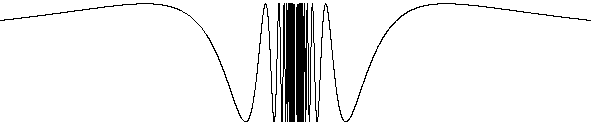
\includegraphics[scale=0.5]{fig/sin1x.pdf}};
\draw (4,1.4)node{$y=\sin\left(\frac1x\right)$};
\end{tikzpicture}
 \hfill
\pause
\begin{tikzpicture}[scale=0.5]
  \draw[->] (-2.2,0) -- (2.2,0) node[right] {$x$};
  \draw[->] (0,0) -- (0,4.2) node[above] {$y$};
\draw[step=1cm, ultra thin] (-2,0) grid (2,4);
   \draw[scale=1,domain=-2:2,smooth,variable=\x,C2, ultra thick] plot ({\x},{\x*\x}) node[below right]{$y=x^2$};     \end{tikzpicture}

\pause
\only<beamer>{\begin{center}
\begin{tikzpicture}
\myaxis{x}{3}{3}{y}{1}{1}
\draw (0,0) node{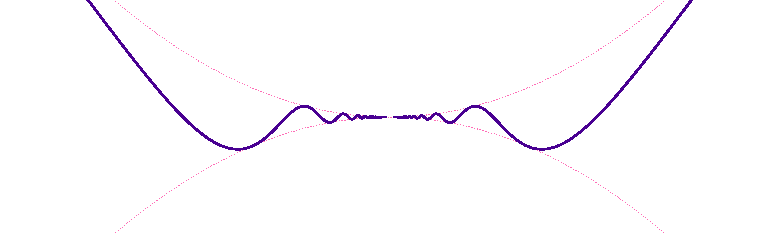
\includegraphics[height=2cm]{fig/x2sin1x.pdf}};
\draw (3,.75)node[right]{$y=x^2\sin\left(\frac1x\right)$};
\end{tikzpicture}
\end{center}}
\MoreSpace
\unote{Example~\eref{text}{eg_1_4_8}}
\end{frame}
 %--------
%----------------------------------------------------------------------------------------
\begin{frame}[t]
$\dlimx{0}x^2\sin\left(\frac{1}{x}\right)$\vfill\pause
\begin{align*}
\textcolor{M5}{-1}&& \leq &&\textcolor{C3}{\sin\left(\frac{1}{x}\right)} &&\leq&& \textcolor{C4}{1}\\
\answer{\mbox{so~~~}\textcolor{M5}{ -x^2}&& \leq &&\textcolor{C3}{x^2\sin\left(\frac{1}{x}\right)}&& \leq&& \textcolor{C4}{x^2}\\
\mbox{and also~~~}\textcolor{M5}{ \dlimx{0}{-x^2}}&&=&&0&&=&&\textcolor{C4}{\dlimx{0}x^2}}\end{align*}
\pause\vfill
\answer{Therefore, by the Squeeze Theorem, $\textcolor{C3}{\dlimx{0}x^2\sin\left(\frac{1}{x}\right)}=0$.}\vfill
\unote{Example~\eref{text}{eg_1_4_8}}
\end{frame}
%----------------------------------------------------------------------------------------
 %--------
%---------------------------------------------------------------------------------------
